\documentclass[abstract, english]{scrartcl}
\addtokomafont{disposition}{\boldmath}

% LuaLatex
% \usepackage{polyglossia}
% \setmainlanguage{english}

% \usepackage{fontspec}
% \setmainfont[
%     Ligatures=TeX,
%     SmallCapsFont={Latin Modern Roman Caps},
%     SlantedFont={* Slanted},
%     ItalicFeatures  = {
%         SmallCapsFont = {LMRomanCaps10-Oblique}
%     },
%     ]{Latin Modern Roman}

% pdflatex
\usepackage[english]{babel}
\usepackage[T1]{fontenc}
\usepackage[utf8]{inputenc}
\usepackage{lmodern}

\usepackage{microtype}

\usepackage{todonotes}
\usepackage{blindtext}

\usepackage{amsmath}
\usepackage{amssymb}
\usepackage{mathdots}
\usepackage{mathtools}
\usepackage{csquotes}
\usepackage{enumitem}

\usepackage{subcaption}
\usepackage[font=small, labelfont=bf, format=hang, indention=-2em]{caption}

\usepackage{algorithm}
\usepackage[noend]{algpseudocode}

\usepackage[hyperref,thmmarks,amsmath]{ntheorem}

\usepackage{url}
\usepackage[pdftex, hypertexnames=false, unicode]{hyperref}
\usepackage[nameinlink, noabbrev]{cleveref}

\usepackage{tikz}
\usepackage{pgfplots}
\pgfplotsset{compat=1.12}
\usetikzlibrary{calc}

%%%

\theoremstyle{plain}
\theoremheaderfont{\rmfamily\bfseries\upshape\boldmath}
\theorembodyfont{\itshape}
\theoremseparator{}
\theoremsymbol{}
\newtheorem{definition}{Definition}
\newtheorem{theorem}[definition]{Theorem}
\newtheorem{lemma}[definition]{Lemma}
\newtheorem{problem}[definition]{Problem}
\newtheorem{observation}[definition]{Observation}

\theoremstyle{plain}
\theoremheaderfont{\scshape}
\theorembodyfont{}
\theoremseparator{}
\theoremsymbol{\qed}
\newtheorem*{proof}{Proof}

\theoremstyle{break}
\theoremheaderfont{\rmfamily\bfseries\upshape\boldmath}
\theorembodyfont{}
\theoremseparator{}
\theoremsymbol{}
\newtheorem{Algorithm}[definition]{Algorithm}

\crefname{observation}{observation}{observations}
\Crefname{observation}{Observation}{Observations}
\crefname{Algorithm}{algorithm}{algorithms}
\Crefname{Algorithm}{Algorithm}{Algorithms}

%%%

\newcommand{\R}{\mathbb{R}}
\newcommand{\Ha}{\mathcal{H}}
\newcommand{\F}{\mathcal{F}}
\newcommand{\Ge}{\mathcal{G}}
\newcommand{\Oh}{\mathcal{O}}

\DeclareMathOperator{\dist}{d}
\DeclareMathOperator{\pow}{pow}
\DeclareMathOperator{\PD}{PD}
\DeclareMathOperator{\cell}{cell}
\DeclareMathOperator{\chor}{chor}
\DeclareMathOperator{\aff}{aff}
\DeclareMathOperator{\CH}{CH}
\DeclareMathOperator{\CHb}{CH_b}
\DeclareMathOperator{\CHt}{CH_t}
\DeclareMathOperator{\IL}{IL}
\DeclareMathOperator{\ls}{ls}
\DeclareMathOperator{\Time}{T}

\newcommand{\abs}[1]{\left\vert #1 \right\vert}
\newcommand{\norm}[1]{\left\Vert #1 \right\Vert}
\newcommand{\scalar}[1]{\left\langle #1 \right\rangle}
\newcommand{\powerset}[1]{\mathcal{P}(#1)}

\newcommand{\define}[1]{\emph{#1}}

\newcommand{\Wlog}{w.\,l.\,o.\,g.\ }
\newcommand{\WLOG}{W.\,l.\,o.\,g.\ }

% From llncs.cls
\def\squareforqed{\hbox{\rlap{$\sqcap$}$\sqcup$}}
\def\qed{\ifmmode\squareforqed\else{\unskip\nobreak\hfil \penalty50\hskip1em\null\nobreak\hfil\squareforqed \parfillskip=0pt\finalhyphendemerits=0\endgraf}\fi}

% See https://tex.stackexchange.com/questions/4302/prettiest-way-to-typeset-c-cplusplus
\def\CC{{C\nolinebreak[4]\hspace{-.05em}\raisebox{.4ex}{\tiny\textbf{++}}}\xspace}

\xdefinecolor{tumblue}     {RGB}{  0,101,189}
\xdefinecolor{tumgreen}    {RGB}{162,173,  0}
\xdefinecolor{tumred}      {RGB}{229, 52, 24}
\xdefinecolor{tumivory}    {RGB}{218,215,203}
\xdefinecolor{tumorange}   {RGB}{227,114, 34}
\xdefinecolor{tumlightblue}{RGB}{152,198,234}

\tikzstyle{every node} = [font=\normalsize]

\tikzstyle{edge} = [very thick]
\tikzstyle{internal edge} = [edge, tumorange]
\tikzstyle{extremal edge} = [edge, tumgreen]
\tikzstyle{node on edge} = [fill=white, circle, inner sep=1pt, font=\small]
\tikzstyle{internal spheres} = [node on edge]
\tikzstyle{extremal spheres} = [node on edge, very near start]

\tikzstyle{sphere center} = [tumred]
\tikzstyle{sphere radius} = [thin, scale=0.5]
\tikzstyle{point} = [circle, draw, fill, minimum size=4pt, inner sep=0pt]


\title{Inzidenz-Strukturen von Powerdiagrammen}
\subtitle{Interdisziplinäres Projekt}
\author{\href{mailto:markus.kaiser@in.tum.de}{Markus Kaiser}}
\date{5. Oktober 2015}

\begin{document}

\begin{frame}
    \titlepage
\end{frame}

\begin{frame}
    \frametitle{Voronoi- und Powerdiagramme}

    \centering
    \begin{tikzpicture}
        \path[use as bounding box] (-4, -3.05) rectangle (7, 5.05);
        \path[clip] (-5, -3.05) rectangle (7.5, 5.05);

        \node[sphere center, label={above:$s_1$}] (s1) at (     2.0,     3.0) {};
        \node[sphere center, label={above:$s_5$}] (s2) at (     5.0,     0.0) {};
        \node[sphere center, label={above:$s_3$}] (s3) at (    -2.0,     0.0) {};
        \node[sphere center, label={below:$s_4$}] (s4) at (     2.0,     0.0) {};
        \node[sphere center, label={above:$s_2$}] (s5) at (     4.0,     2.0) {};

        \coordinate (p1v) at (     0.0,     1.5);
        \coordinate (p2v) at (     3.5,     0.5);
        \coordinate (p3v) at (     2.5,     1.5);

        \coordinate (p1) at (   0.625,     2.0);
        \coordinate (p2) at (     4.0,    0.75);
        \coordinate (p3) at (    2.75,     2.0);

        \only<2-3> {
            \draw[thin] (s4) edge (s2);
            \draw[thin] (s4) edge (s1);
            \draw[right angle length=1.5ex, right angle symbol={s4}{s2}{p2v}];
            \draw[right angle length=1.5ex, right angle symbol={s4}{s1}{p3v}];

            \draw[internal edge] (p1v) edge node[internal spheres] {${1, 4}$} (p3v);
            \draw[extremal edge] (p2v) edge node[extremal spheres] {${4, 5}$} ($(p2v) + 10*(     0.0,    -1.0)$);
        }

        \only<3> {
            \draw[internal edge] (p2v) edge node[internal spheres] {${2, 4}$} (p3v);
            \draw[extremal edge] (p1v) edge node[extremal spheres] {${3, 4}$} ($(p1v) + 10*(    -0.0,    -1.0)$);
            \draw[extremal edge] (p1v) edge node[extremal spheres] {${1, 3}$} ($(p1v) + 10*(    -0.6,     0.8)$);
            \draw[extremal edge] (p2v) edge node[extremal spheres] {${2, 5}$} ($(p2v) + 10*(  0.8944,  0.4472)$);
            \draw[extremal edge] (p3v) edge node[extremal spheres] {${1, 2}$} ($(p3v) + 10*(  0.4472,  0.8944)$);

            \node[point] () at (p1v) {};
            \node[point] () at (p2v) {};
            \node[point] () at (p3v) {};
        }

        \only<4-5> {
            \draw[sphere radius] (s1) circle[radius=1.0];
            \draw[sphere radius] (s2) circle[radius=1.0];
            \draw[sphere radius] (s3) circle[radius=3.0];
            \draw[sphere radius] (s4) circle[radius=2.0];
            \draw[sphere radius] (s5) circle[radius=1.0];
        }

        \only<5> {
            \draw[thin] (s4) edge (s2);
            \draw[right angle length=1.5ex, right angle symbol={s4}{s2}{p2}];
            % \draw[thin]
            %     (s4) edge (s5)
            %     (s4) edge (s2)
            %     (s2) edge (s5);
            % \draw[right angle length=1.5ex, right angle symbol={s4}{s5}{p2}];
            % \draw[right angle length=1.5ex, right angle symbol={s4}{s2}{p2}];
            % \draw[right angle length=1.5ex, right angle symbol={s2}{s5}{p2}];

            \draw[extremal edge] (p1) edge node[extremal spheres] {${1, 3}$} ($(p1) + 10*(    -0.6,     0.8)$);
            \draw[extremal edge] (p1) edge node[extremal spheres, pos=0.2] {${3, 4}$} ($(p1) + 10*(     0.0,    -1.0)$);
            \draw[internal edge] (p1) edge node[internal spheres, pos=0.2] {${1, 4}$} (p3);
            \draw[extremal edge] (p2) edge node[extremal spheres, pos=0.2] {${4, 5}$} ($(p2) + 10*(    -0.0,    -1.0)$);
            \draw[extremal edge] (p2) edge node[extremal spheres] {${2, 5}$} ($(p2) + 10*(  0.8944,  0.4472)$);
            \draw[internal edge] (p2) edge node[internal spheres, pos=0.5] {${2, 4}$} (p3);
            \draw[extremal edge] (p3) edge node[extremal spheres] {${1, 2}$} ($(p3) + 10*(  0.4472,  0.8944)$);

            \node[point] () at (p1) {};
            \node[point] () at (p2) {};
            \node[point] () at (p3) {};
        }
    \end{tikzpicture}
\end{frame}

\begin{frame}
    \frametitle{Power-Funktion}

    \begin{definition}[Power-Funktion]
        Die \structure{Power} eines Punktes $x \in \R^d$ in Bezug zu einer Sphäre $s$ mit Zentrum $z \in \R^d$ und Radius $r \geq 0$ ist
        \begin{align}
            \pow(x, s) = \dist(x, z)^2 - r^2.
        \end{align}
    \end{definition}

    \centering
    \begin{tikzpicture}[x=1cm, y=1cm]
        \coordinate (center) at (0, 0);
        \coordinate (point) at (2, 3);

        \node[power circle, minimum size=3cm, label={[yshift=0.5cm]below:$s$}] (circle) at (center) {};

        \coordinate (tangent) at (tangent cs:node=circle,point={(point)},solution=1);

        \draw[right angle length=1.5ex, right angle symbol={center}{tangent}{point}];

        \draw
        (tangent) edge[black] node[midway, left] {$r$} (center.center)
        (center.center) edge[black] node[pos=0.6, sloped, below] {$\dist(x, z)$} (point)
        (point) edge[very thick, tumblue] node[midway, sloped, above] {$\pow(x, s)$} (tangent);
        \draw
        (center)
        node[power center, label={below:$z$}] () {}

        (point)
        node[power point, label={above:$x$}] () {};
    \end{tikzpicture}
\end{frame}

\begin{frame}
    \frametitle{Eigenschaften von Powerdiagrammen}

    \centering
    \begin{tikzpicture}[x=0.5cm, y=0.5cm]
        \path[use as bounding box] (-4, -9) rectangle (18, 8);
        \path[clip] (-6, -9) rectangle (19, 8);

        \node[sphere center, label={above:$s_5$}] (s1) at (    10.0,     4.0) {};
        \draw[sphere radius] (s1) circle[radius=3.5];
        \node[sphere center, label={right:$s_3$}] (s2) at (    15.0,    -3.0) {};
        \draw[sphere radius] (s2) circle[radius=3.2];
        \node[sphere center, label={left:$s_1$}] (s3) at (     0.0,     0.0) {};
        \draw[sphere radius] (s3) circle[radius=5.0];
        \node[sphere center, label={above:$s_4$}] (s4) at (    13.5,    -3.0) {};
        \draw[sphere radius] (s4) circle[radius=1.3];
        \node[sphere center, label={above:$s_2$}] (s5) at (    1.7,    0) {};
        \draw[sphere radius] (s5) circle[radius=1.5];

        \coordinate (p1) at (   7.408,  -2.425);
        \coordinate (p2) at (    11.4, -0.4293);

        \draw[extremal edge] (p1) edge node[extremal spheres, pos=0.3] {${1, 5}$} ($(p1) + 15*( -0.3714,  0.9285)$);
        \draw[extremal edge] (p1) edge node[extremal spheres, pos=0.2] {${1, 4}$} ($(p1) + 15*( -0.2169, -0.9762)$);
        \draw[internal edge] (p1) edge node[internal spheres] {${4, 5}$} (p2);
        \draw[extremal edge] (p2) edge node[extremal spheres, pos=0.3] {${3, 5}$} ($(p2) + 15*(  0.8137,  0.5812)$);
        \draw[extremal edge] (p2) edge node[extremal spheres, pos=0.3] {${3, 4}$} ($(p2) + 15*(    -0.0,    -1.0)$);

        \node[point] () at (p1) {};
        \node[point] () at (p2) {};
    \end{tikzpicture}
\end{frame}

\begin{frame}<-4>[label=transformation]
    \frametitle{Transformationsfunktion}

    \centering
    \begin{tikzpicture}[y=0.80pt, x=0.80pt, yscale=-0.8, xscale=1, inner sep=0pt, outer sep=0pt,font=\scriptsize]
        \begin{scope}[cm={{1.25,0.0,0.0,-1.25,(0.0,900.0)}}]
            \path[use as bounding box] (100, 60) rectangle (390, 360);
            % Paraboloid
            \only<2-6> {
                \path[draw=black,line join=miter,line cap=butt,miter limit=4.00,even odd
                rule] (212.3294,187.2000) .. controls (217.7922,182.5589)
                and (223.8195,178.2548) .. (230.5412,175.7647) .. controls (231.5379,175.3954)
                and (232.5544,175.0498) .. (233.5853,174.7367)(193.2706,208.8000) .. controls
                (198.8151,200.9605) and (205.0117,193.4170) ..
                (212.3294,187.2000)(174.6353,242.2588) .. controls (180.4241,230.8806) and
                (185.8991,219.2228) .. (193.2706,208.8000)(156.4235,281.6471) .. controls
                (156.4235,281.6471) and (168.0762,255.1511) ..
                (174.6353,242.2588)(164.3483,275.2060) .. controls (161.8204,276.4974) and
                (159.0551,277.8363) .. (157.4186,280.1557)(180.3289,269.8319) .. controls
                (174.8947,271.2652) and (169.3529,272.6491) ..
                (164.3483,275.2060)(207.3404,264.5994) .. controls (198.2234,265.5950) and
                (189.1968,267.4930) .. (180.3289,269.8319)(239.7259,263.7508) .. controls
                (228.9290,263.5424) and (218.0754,263.4271) ..
                (207.3404,264.5994)(276.7783,266.1550) .. controls (264.4832,264.7351) and
                (252.1003,263.9897) .. (239.7259,263.7508)(281.1507,266.6821) .. controls
                (279.6937,266.4945) and (278.2348,266.3232) ..
                (276.7783,266.1550)(312.1336,300.9447) .. controls (313.2517,300.4916) and
                (314.4024,300.0643) .. (315.5357,299.6013)(306.1939,302.7831) .. controls
                (308.1905,302.2270) and (310.2127,301.7230) ..
                (312.1336,300.9447)(288.5162,307.1672) .. controls (294.4892,306.0805) and
                (300.3454,304.4120) .. (306.1939,302.7831)(258.3935,310.7027) .. controls
                (268.4813,310.0354) and (278.5696,308.9768) ..
                (288.5162,307.1672)(239.8673,310.9856) .. controls (246.0434,310.9786) and
                (252.2308,311.1104) .. (258.3935,310.7027)(229.1192,310.8441) .. controls
                (232.6966,311.0448) and (236.2843,310.9893) ..
                (239.8673,310.9856)(210.5930,309.0057) .. controls (216.7204,309.9886) and
                (222.9233,310.4966) .. (229.1192,310.8441)(183.2987,302.9245) .. controls
                (192.1948,305.7073) and (201.3895,307.5292) ..
                (210.5930,309.0057)(164.9139,295.4292) .. controls (170.4128,299.1116) and
                (176.9825,300.9488) .. (183.2987,302.9245)(155.7216,286.0954) .. controls
                (156.8008,290.3267) and (161.2856,292.9994) ..
                (164.9139,295.4292)(157.4186,280.1557) .. controls (156.2316,281.8382) and
                (155.2127,284.1001) .. (155.7216,286.0954);
                \alt<-3>{
                    \path[draw=black,line join=miter,line
                    cap=butt,miter limit=4.00,even odd rule]
                    (317.7882,269.3647) .. controls (319.1527,272.7162) and (320.6622,277.9665) ..
                    (322.6234,282.0431) .. controls (323.2589,283.3640) and (323.8203,284.8492) ..
                    (324.2378,285.9741)(303.8118,237.6000) .. controls (309.0582,247.9097) and
                    (313.4263,258.6508) .. (317.7882,269.3647)(290.2588,214.3059) .. controls
                    (295.1243,221.8575) and (299.7375,229.5937) ..
                    (303.8118,237.6000)(278.8235,198.2118) .. controls (283.1211,203.1958) and
                    (286.6945,208.7737) .. (290.2588,214.3059)(257.2235,177.4588) .. controls
                    (265.5326,182.9953) and (272.3033,190.6500) ..
                    (278.8235,198.2118)(247.4823,173.2235) .. controls (250.9929,173.6847) and
                    (254.2770,175.4955) .. (257.2235,177.4588)(233.5852,174.7367) .. controls
                    (238.0924,173.3674) and (242.8746,172.6182) ..
                    (247.4823,173.2235)(292.9003,268.8420) .. controls (289.0511,267.8226) and
                    (285.1075,267.1918) .. (281.1507,266.6821)(310.5779,275.3474) .. controls
                    (304.9808,272.5020) and (298.9699,270.4494) ..
                    (292.9003,268.8420)(321.1845,282.4185) .. controls (318.2566,279.3390) and
                    (314.3658,277.2730) .. (310.5779,275.3474)(325.5686,289.7724) .. controls
                    (325.6261,286.9191) and (323.1510,284.4866) ..
                    (321.1845,282.4185)(321.3260,296.2777) .. controls (323.2528,294.5487) and
                    (325.5164,292.3607) .. (325.5686,289.7724)(315.5357,299.6013) .. controls
                    (317.6307,298.7453) and (319.6662,297.7671) .. (321.3260,296.2777);
                }{
                    \path[draw=black,dash pattern=on 2.56pt off 2.56pt,line join=miter,line
                    cap=butt,miter limit=4.00,even odd rule]
                    (317.7882,269.3647) .. controls (319.1527,272.7162) and (320.6622,277.9665) ..
                    (322.6234,282.0431) .. controls (323.2589,283.3640) and (323.8203,284.8492) ..
                    (324.2378,285.9741)(303.8118,237.6000) .. controls (309.0582,247.9097) and
                    (313.4263,258.6508) .. (317.7882,269.3647)(290.2588,214.3059) .. controls
                    (295.1243,221.8575) and (299.7375,229.5937) ..
                    (303.8118,237.6000)(278.8235,198.2118) .. controls (283.1211,203.1958) and
                    (286.6945,208.7737) .. (290.2588,214.3059)(257.2235,177.4588) .. controls
                    (265.5326,182.9953) and (272.3033,190.6500) ..
                    (278.8235,198.2118)(247.4823,173.2235) .. controls (250.9929,173.6847) and
                    (254.2770,175.4955) .. (257.2235,177.4588)(233.5852,174.7367) .. controls
                    (238.0924,173.3674) and (242.8746,172.6182) ..
                    (247.4823,173.2235)(292.9003,268.8420) .. controls (289.0511,267.8226) and
                    (285.1075,267.1918) .. (281.1507,266.6821)(310.5779,275.3474) .. controls
                    (304.9808,272.5020) and (298.9699,270.4494) ..
                    (292.9003,268.8420)(321.1845,282.4185) .. controls (318.2566,279.3390) and
                    (314.3658,277.2730) .. (310.5779,275.3474)(325.5686,289.7724) .. controls
                    (325.6261,286.9191) and (323.1510,284.4866) ..
                    (321.1845,282.4185)(321.3260,296.2777) .. controls (323.2528,294.5487) and
                    (325.5164,292.3607) .. (325.5686,289.7724)(315.5357,299.6013) .. controls
                    (317.6307,298.7453) and (319.6662,297.7671) .. (321.3260,296.2777);
                }
            }

            % Intersection lines
            \only<7-> {
                \path[draw=tumorange,line join=miter,line cap=butt,miter limit=4.00,even odd
                rule, very thick] (197.6000,66.9429) -- (285.6023,132.8780);
                \path[draw=tumorange,line join=miter,line cap=butt,miter limit=4.00,even odd
                rule, very thick] (226.1189,145.9960) -- (344.9903,252.5778);
            }

            % x1-x2-plane
            \path[draw=black,line join=miter,line cap=butt,miter limit=4.00,even odd
            rule] (197.6000,66.9429) -- (104.1428,66.9429);
            \path[draw=black, arrows={-latex}, line join=miter,line cap=butt,miter
            limit=4.00,even odd rule]
            (141.6447,131.7009) -- (104.1428,66.9429) node[label={left:$x_2$}]{};
            \path[draw=black,line join=miter,line cap=butt,miter limit=4.00,even odd
            rule] (141.6447,131.7009) -- (191.7098,132.1344);
            \path[draw=black,line join=miter,line cap=butt,miter limit=4.00,even odd
            rule] (191.7098,132.1344) -- (222.6000,132.4019);
            \path[draw=black,line join=miter,line cap=butt,miter limit=4.00,even odd
            rule] (367.4572,133.4572) -- (388.2572,66.9429);
            \path[draw=black,line join=miter,line cap=butt,miter limit=4.00,even odd
            rule] (388.2572,66.9429) -- (197.6000,66.9429);
            \path[draw=black, arrows={-latex},line join=miter,line cap=butt,miter limit=4.00,even odd
            rule] (285.6023,132.8780) -- (367.4572,133.4572) node[label={[label distance=.25em]right:$x_1$}]{};
            \path[draw=black,line join=miter,line cap=butt,miter limit=4.00,even odd
            rule] (285.6023,132.8780) -- (257.7040,132.6452);
            \only<-3,8-> {
                \path[draw=black,line join=miter,line cap=butt,miter limit=4.00,even odd
                rule] (222.6,132.4019) -- (285.6000,132.8780);
            }

            % x_3 axis
            \only<2-> {
                \path[draw=black,line join=miter,line cap=butt,miter limit=4.00,nonzero
                rule] (243.1343,101.4316) -- (242.9474,122.0474);
                \path[draw=black,dash pattern=on 4.99pt off 1.25pt on 0.62pt off 1.25pt,line
                join=miter,line cap=butt,miter limit=4.00,nonzero rule]
                (242.9474,122.0473) -- (241.6657,263.4320);
                \path[draw=black,line join=miter,line cap=round,miter limit=4.00,nonzero
                rule,arrows={-latex}] (241.7391,263.9741) -- (241.6638,343.1295) node[label={above:$x_3$}]{};
            }

            % Circles and projections
            \begin{scope}[tumred]
                \path[draw,line join=miter,line cap=round,miter limit=4.00,nonzero
                rule] (195.1641,107.6757) .. controls (195.1476,111.7672)
                and (204.0558,115.0899) .. (215.0665,115.0991) .. controls (226.0773,115.1081)
                and (235.0258,111.8006) .. (235.0589,107.7091)(215.1265,100.2745) .. controls
                (204.1157,100.2715) and (195.1806,103.5841) ..
                (195.1641,107.6757)(235.0589,107.6868) .. controls (235.0589,103.5952) and
                (226.1373,100.2775) .. (215.1265,100.2745);

                \only<3-4> {
                    \path[draw,dash pattern=on 2.56pt off 2.56pt,line join=miter,line
                    cap=butt,miter limit=4.00,nonzero rule] (234.7192,219.6998)
                    .. controls (234.6688,226.2075) and (232.1661,234.6090) ..
                    (227.3925,242.8227)(227.3925,242.8227) .. controls (218.9241,257.3941) and
                    (206.5155,265.8568) .. (199.6773,261.7247) .. controls (196.7369,259.9479) and
                    (195.3057,256.1317) .. (195.3017,251.2001)(195.3017,251.2001) .. controls
                    (195.2967,244.6625) and (197.8020,236.1647) .. (202.6291,227.8589) .. controls
                    (211.0976,213.2875) and (223.5061,204.8248) .. (230.3443,208.9569) .. controls
                    (233.3279,210.7598) and (234.7582,214.6625) .. (234.7192,219.6998);
                }
                \only<3-4> {
                    \path[draw,dash pattern=on 0.64pt off 1.92pt,line join=miter,line
                    cap=butt,miter limit=4.00,nonzero rule] (235.0589,107.7091)
                    -- (234.7192,219.6998);
                    \path[draw,dash pattern=on 0.64pt off 1.92pt,line join=miter,line
                    cap=butt,miter limit=4.00,nonzero rule] (195.3017,251.2001)
                    -- (195.1641,107.6757);
                }
            \end{scope}
            \begin{scope}[tumgreen]
                \path[draw,line join=miter,line cap=round,miter limit=4.00,nonzero
                rule] (248.1028,85.9943) .. controls (248.0787,92.5248) and
                (262.1904,97.6159) .. (278.2344,97.6306) .. controls (294.2784,97.6453) and
                (305.8324,92.6134) .. (305.8806,86.0830)(305.8807,86.0298) .. controls
                (305.8807,79.4994) and (294.3658,73.9743) .. (278.3218,73.9694) .. controls
                (262.2777,73.9645) and (248.1250,79.4557) .. (248.1009,85.9861);

                \only<3-4> {
                    \path[draw,line join=miter,line cap=round,miter limit=4.00,nonzero
                    rule] (306.0247,258.7996) .. controls (306.0083,260.9460)
                    and (305.5164,262.6311) .. (304.5000,263.7327) .. controls (299.3848,269.2763)
                    and (282.9214,257.9415) .. (267.7278,238.4156) .. controls (255.8617,223.1661)
                    and (248.2796,207.4304) .. (247.9645,198.6286)(306.0247,258.7996) .. controls
                    (306.0909,250.1440) and (298.4260,233.9864) .. (286.2515,218.3406) .. controls
                    (271.0580,198.8148) and (254.5946,187.4799) .. (249.4794,193.0235) .. controls
                    (248.3591,194.2376) and (247.8761,196.1605) .. (247.9645,198.6286);
                }
                \only<3-4> {
                    \path[draw,dash pattern=on 0.64pt off 1.92pt,line join=miter,line
                    cap=butt,miter limit=4.00,nonzero rule] (247.9645,198.6286)
                    -- (248.1028,85.9943);
                    \path[draw,dash pattern=on 0.64pt off 1.92pt,line join=miter,line
                    cap=round,miter limit=4.00,nonzero rule] (305.8806,86.0830)
                    -- (306.0247,258.7995);
                }
            \end{scope}

            % Pi planes
            \only<4-> {
                \begin{scope}[black, onslide={<4-5> tumgreen}]
                    \path[draw,thick,line join=miter,line cap=butt,miter limit=4.00,even odd
                    rule] (226.1189,145.9960) --
                    (249.8835,236.6651)(371.2821,352.8979) --
                    (344.9903,252.5778)(249.8835,236.6651) --
                    (371.2821,352.8979);
                \end{scope}
                \begin{scope}[black, onslide={<4-5> tumred}]
                    \path[draw,thick,line join=miter,line cap=butt,miter limit=4.00,even odd
                    rule] (226.1189,145.9960) -- (157.1446,243.8588);
                    \path[draw,thick,line join=miter,line cap=butt,miter limit=4.00,even odd
                    rule] (157.1446,243.8588) -- (169.1107,253.7846);
                    \path[draw,thick,line join=miter,line cap=butt,miter limit=4.00,even odd
                    rule] (238.0256,310.9489) -- (279.5673,345.4074);
                    \path[draw,thick,line join=miter,line cap=butt,miter limit=4.00,even odd
                    rule] (279.5673,345.4074) -- (313.3697,297.4475);

                    \only<4-5, 7-> {
                        \path[draw,thick,dash pattern=on 2.56pt off 2.56pt,line join=miter,line
                        cap=butt,miter limit=4.00,even odd rule]
                        (313.3697,297.4475) -- (344.9903,252.5778);
                    }

                    \alt<-6> {
                        \path[draw,thick,dash pattern=on 2.56pt off 2.56pt,line join=miter,line
                        cap=butt,miter limit=4.00,even odd rule]
                        (169.1107,253.7846) -- (238.0256,310.9489);
                    }{
                        \path[draw,thick,line join=miter,line
                        cap=butt,miter limit=4.00,even odd rule]
                        (169.1107,253.7846) -- (238.0256,310.9489);
                    }
                \end{scope}

                \only<-7> {
                    \begin{scope}[black, onslide={<4-5> tumgreen}]
                        \path[draw,thick,dash pattern=on 2.56pt off 2.56pt,line join=miter,line
                        cap=butt,miter limit=4.00,even odd rule]
                        (287.8263,176.7128) -- (238.0560,129.0592)(337.5966,224.3664) --
                        (287.8263,176.7128)(344.9903,252.5778) -- (337.5966,224.3664);
                        \path[draw,thick,line join=miter,line cap=butt,miter limit=4.00,even odd
                        rule]
                        (238.0560,129.0592) -- (216.1980,108.1336) -- (226.1189,145.9960);
                    \end{scope}
                    \begin{scope}[black, onslide={<4-5> tumred}]
                        \path[draw,thick,line join=miter,line cap=butt,miter limit=4.00,even odd
                        rule] (257.7040,132.6452) -- (243.7156,121.0292);
                        \path[draw,thick,line join=miter,line cap=butt,miter limit=4.00,even odd
                        rule] (238.0560,129.0592) -- (235.5971,132.5480);
                        \path[draw,thick,line join=miter,line cap=butt,miter limit=4.00,even odd
                        rule] (235.5971,132.5480) -- (226.1189,145.9960);
                        \path[draw,thick,line join=miter,line cap=butt,miter limit=4.00,even odd
                        rule] (344.9903,252.5778) -- (366.1384,222.5777);
                        \path[draw,thick,line join=miter,line cap=butt,miter limit=4.00,even odd
                        rule] (366.1384,222.5777) -- (257.7040,132.6452);
                        \path[draw,thick,line join=miter,line cap=butt,miter limit=4.00,even odd
                        rule] (243.7156,121.0292) -- (238.0560,129.0592);
                    \end{scope}
                }
            }

            % Projection point
            \coordinate (p1)   at (295, 115);
            \coordinate (p1p1) at (295, 170);
            \coordinate (p1p2) at (295, 215);
            \coordinate (p1u)  at (295, 295);

            \only<5-6> {
                \path[draw=tumblue,dash pattern=on 0.64pt off 1.92pt,line join=miter,line
                cap=butt,miter limit=4.00,nonzero rule]
                    (p1) -- (p1u);

                \tikzstyle{intersection} = [sphere center, tumblue, minimum size=2pt];
                \node[intersection, minimum size=4pt, label={[yshift=-0.3ex]below:$p$}] at (p1) {};
                \node[intersection, tumred] at (p1p1) {};
                \node[intersection, tumgreen] at (p1p2) {};
                \node[intersection, black] at (p1u) {};
            }

            \only<6> {
                \draw[thick, tumred]
                    ($(p1p1) - (0.3em, 0)$) --
                    ($(p1u) - (0.3em, 0)$)
                    node[pos=0.2, label={left:$\pow(p, s_1)$}] {};

                \draw[thick, tumgreen]
                    ($(p1p2) + (0.3em, 0)$) --
                    ($(p1u) + (0.3em, 0)$)
                    node[pos=0.6, label={right:$\pow(p, s_2)$}] {};
            }

            \only<4-> {
                \node at (375, 285) {$\Pi(s_2)$};
                \node at (165, 200) {$\Pi(s_1)$};
            }

            \node at (200, 96) {$s_1$};
            \node at (250, 73) {$s_2$};
        \end{scope}
    \end{tikzpicture}
\end{frame}

\begin{frame}[t]
    \frametitle{Transformationsfunktion}

    Sei $s = (z, r^2)$ eine Sphäre und $x$ ein Punkt im Originalraum.
    \vfill
    \begin{lemma}
        Sei \structure{$\pi_U$} die vertikale Projektion von $x$ auf den Paraboloiden und\\
        sei \structure{$\pi_s$} die Projektion auf $\Pi(s)$.\\
        Dann ist die \structure{Power-Funktion} von $x$ und $s$ gegeben durch
        \begin{align}
            \pow(x, s) = \dist(x, \pi_U) - \dist(x, \pi_s).
        \end{align}
    \end{lemma}
    \vfill
\end{frame}

\againframe<4->{transformation}

\begin{frame}
    \frametitle{Powerdiagramme und Polyeder}

    \begin{theorem}
        Zu \structure{jedem $(d+1)$-Polyeder}, der \structure{nur nach unten} beschränkt ist, existiert ein äquivalentes Powerdiagramm in $d$ Dimensionen und umgekehrt.
    \end{theorem}
\end{frame}

\begin{frame}[label=polarisation]
    \frametitle{Polarisationsfunktion}

    \centering
    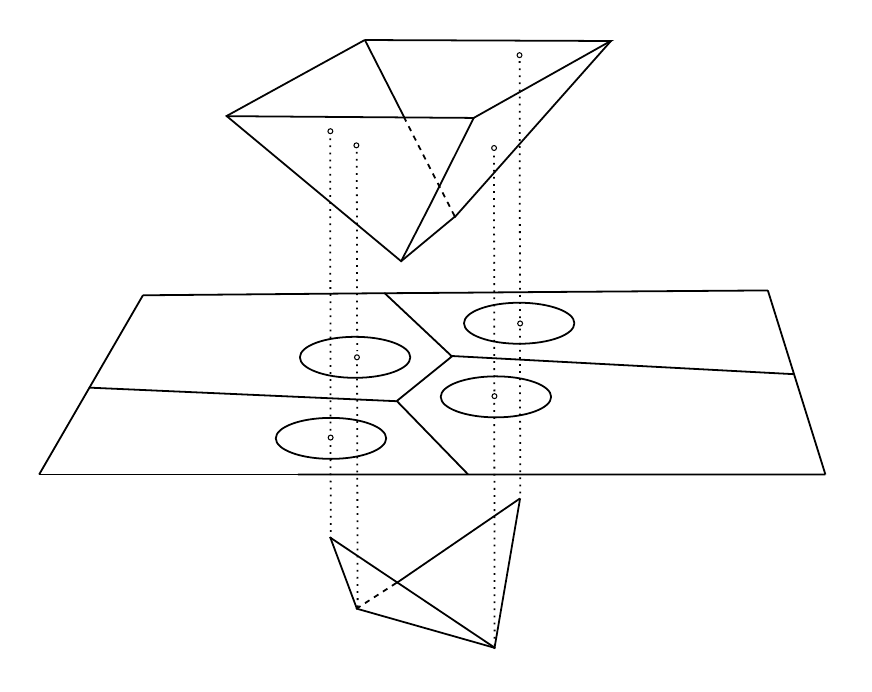
\begin{tikzpicture}[y=0.80pt, x=0.80pt, yscale=-1.000000, xscale=1.000000, inner sep=0pt, outer sep=0pt]
        \begin{scope}[cm={{1.25,0.0,0.0,-1.25,(0.0,900.0)}}]
            \path[use as bounding box] (100, 240) rectangle (395, 470);

            % Spheres
            \path[xscale=1.000,yscale=-1.000,line join=miter,line cap=round,miter
            limit=4.00,fill opacity=0.000,nonzero rule,line width=0.640pt]
            (221.8826,-454.9180) ellipse (0.9682cm and 1.2072cm);
            \path[draw=black,line join=miter,line cap=round,miter limit=4.00,nonzero
            rule,line width=0.640pt] (198.3641,350.8757) .. controls (198.3476,354.9672)
            and (207.2558,358.2899) .. (218.2665,358.2991) .. controls (229.2773,358.3081)
            and (238.2258,355.0006) .. (238.2588,350.9091)(218.3265,343.4745) .. controls
            (207.3157,343.4715) and (198.3806,346.7841) ..
            (198.3641,350.8757)(238.2589,350.8868) .. controls (238.2589,346.7952) and
            (229.3373,343.4775) .. (218.3265,343.4744);
            \path[draw=black,line join=miter,line cap=round,miter limit=4.00,nonzero
            rule,line width=0.640pt] (189.6526,321.5889) .. controls (189.6361,325.6804)
            and (198.5443,329.0031) .. (209.5550,329.0124) .. controls (220.5658,329.0214)
            and (229.5143,325.7138) .. (229.5473,321.6223)(209.6150,314.1877) .. controls
            (198.6042,314.1847) and (189.6691,317.4974) ..
            (189.6526,321.5889)(229.5474,321.6000) .. controls (229.5474,317.5085) and
            (220.6258,314.1907) .. (209.6150,314.1877);
            \path[draw=black,line join=miter,line cap=round,miter limit=4.00,nonzero
            rule,line width=0.640pt] (257.6526,363.1889) .. controls (257.6361,367.2804)
            and (266.5442,370.6031) .. (277.5550,370.6123) .. controls (288.5658,370.6214)
            and (297.5143,367.3138) .. (297.5473,363.2223)(277.6150,355.7877) .. controls
            (266.6042,355.7847) and (257.6691,359.0974) ..
            (257.6526,363.1889)(297.5474,363.2000) .. controls (297.5474,359.1085) and
            (288.6258,355.7907) .. (277.6150,355.7877);
            \path[draw=black,line join=miter,line cap=round,miter limit=4.00,nonzero
            rule,line width=0.640pt] (249.2526,336.5889) .. controls (249.2361,340.6804)
            and (258.1442,344.0031) .. (269.1550,344.0124) .. controls (280.1658,344.0214)
            and (289.1143,340.7138) .. (289.1473,336.6223)(269.2150,329.1877) .. controls
            (258.2042,329.1847) and (249.2691,332.4974) ..
            (249.2526,336.5889)(289.1474,336.6000) .. controls (289.1474,332.5085) and
            (280.2258,329.1907) .. (269.2150,329.1877);

            % Chordals
            \path[draw=black,line join=miter,line cap=butt,even odd rule,line width=0.648pt]
            (122.1463,339.9370) --
            (233.4649,335.0255) -- (259.0922,308.6262)
            (252.6000,351.4000) -- (376.8000,344.8000)
            (233.3996,335.1217) -- (253.3085,351.2179) --
            (228.8500,374.2000);

            % Plane
            \path[draw=black,line join=miter,line cap=butt,miter limit=4.00,even odd
            rule,line width=0.640pt] (197.6000,308.5429) -- (104.1428,308.5429);
            \path[draw=black,line join=miter,line cap=butt,even odd rule,line width=0.648pt]
            (285.6023,374.4780) -- (257.7040,374.2452) --
            (230.8492,374.0590) -- (222.6000,374.0018) --
            (191.7098,373.7344)
            (367.4572,375.0572) -- (285.6023,374.4780)
            (388.2572,308.5429) -- (241.5477,308.5429) --
            (197.6000,308.5429)
            (367.4572,375.0572) -- (388.2572,308.5429)
            (141.6447,373.3009) -- (191.7098,373.7344)
            (104.1428,308.5429) -- (141.6447,373.3009);

            % Primal polyhedron
            \path[draw=black,opacity=0.990,line join=miter,line cap=butt,even odd rule,line
            width=0.640pt] (171.8713,438.0310) -- (261.1692,437.3901) --
            (245.9441,407.0247);
            \path[draw=black,opacity=0.990,line join=miter,line cap=butt,even odd rule,line
            width=0.640pt] (245.9941,407.0997) -- (234.9553,385.6223);
            \path[draw=black,opacity=0.990,line join=miter,line cap=butt,even odd rule,line
            width=0.640pt] (261.0000,437.3000) -- (310.6665,465.1914) --
            (221.7963,465.5408);
            \path[draw=black,opacity=0.990,line join=miter,line cap=butt,even odd rule,line
            width=0.640pt] (254.2589,401.4621) -- (310.8795,465.3198);
            \path[draw=black,opacity=0.990,line join=miter,line cap=butt,even odd rule,line
            width=0.640pt] (221.8288,465.5646) -- (171.8763,438.0841) --
            (234.9472,385.6085) -- (254.4397,401.7799);
            \path[draw=black,line join=miter,line cap=butt,even odd rule,line width=0.640pt]
            (221.8125,465.6000) -- (236.0500,437.6500);
            \path[draw=black,dash pattern=on 1.92pt off 1.92pt,line join=miter,line
            cap=butt,miter limit=4.00,even odd rule,line width=0.640pt]
            (235.9000,437.8000) -- (254.3500,401.7500);

            % Centers
            \path[xscale=1.000,yscale=-1.000,draw=black,opacity=0.990,line join=miter,line
            cap=butt,miter limit=4.00,nonzero rule,line width=0.379pt]
            (218.9818,-350.8998) ellipse (0.0248cm and 0.0252cm);
            \path[xscale=1.000,yscale=-1.000,draw=black,opacity=0.990,line join=miter,line
            cap=butt,miter limit=4.00,nonzero rule,line width=0.379pt]
            (209.4693,-321.8896) ellipse (0.0248cm and 0.0252cm);
            \path[xscale=1.000,yscale=-1.000,draw=black,opacity=0.990,line join=miter,line
            cap=butt,miter limit=4.00,nonzero rule,line width=0.379pt]
            (268.6725,-336.8510) ellipse (0.0248cm and 0.0252cm);
            \path[xscale=1.000,yscale=-1.000,draw=black,opacity=0.990,line join=miter,line
            cap=butt,miter limit=4.00,nonzero rule,line width=0.379pt]
            (277.9486,-363.1182) ellipse (0.0248cm and 0.0252cm);
            \path[xscale=1.000,yscale=-1.000,draw=black,opacity=0.990,line join=miter,line
            cap=butt,miter limit=4.00,nonzero rule,line width=0.379pt]
            (268.5288,-426.5256) ellipse (0.0248cm and 0.0252cm);
            \path[xscale=1.000,yscale=-1.000,draw=black,opacity=0.990,line join=miter,line
            cap=butt,miter limit=4.00,nonzero rule,line width=0.379pt]
            (277.7205,-460.0618) ellipse (0.0248cm and 0.0252cm);
            \path[xscale=1.000,yscale=-1.000,draw=black,opacity=0.990,line join=miter,line
            cap=butt,miter limit=4.00,nonzero rule,line width=0.379pt]
            (209.3793,-432.5914) ellipse (0.0248cm and 0.0252cm);
            \path[xscale=1.000,yscale=-1.000,draw=black,opacity=0.990,line join=miter,line
            cap=butt,miter limit=4.00,nonzero rule,line width=0.379pt]
            (218.7776,-427.4814) ellipse (0.0248cm and 0.0252cm);

            % Vertical Lines
            \path[draw=black,dash pattern=on 0.64pt off 1.92pt,line join=miter,line
            cap=butt,miter limit=4.00,nonzero rule,line width=0.640pt] (218.9199,425.1651)
            -- (219.0592,353.1356);
            \path[draw=black,dash pattern=on 0.64pt off 1.92pt,line join=miter,line
            cap=butt,miter limit=4.00,nonzero rule,line width=0.640pt] (268.4980,423.7383)
            -- (268.6369,337.7254);
            \path[draw=black,dash pattern=on 0.64pt off 1.92pt,line join=miter,line
            cap=butt,miter limit=4.00,nonzero rule,line width=0.640pt] (209.3102,430.0148)
            -- (209.4484,322.4933);
            \path[draw=black,dash pattern=on 0.64pt off 1.92pt,line join=miter,line
            cap=butt,miter limit=4.00,nonzero rule,line width=0.640pt] (277.7626,457.8852)
            -- (277.9013,364.4477);
            \path[draw=black,dash pattern=on 0.64pt off 1.92pt,line join=miter,line
            cap=butt,miter limit=4.00,nonzero rule,line width=0.640pt] (219.0202,348.3148)
            -- (219.2311,259.8481);
            \path[draw=black,dash pattern=on 0.64pt off 1.92pt,line join=miter,line
            cap=butt,miter limit=4.00,nonzero rule,line width=0.640pt] (268.5988,334.3894)
            -- (268.7376,245.1763);
            \path[draw=black,dash pattern=on 0.64pt off 1.92pt,line join=miter,line
            cap=butt,miter limit=4.00,nonzero rule,line width=0.640pt] (209.4100,319.1627)
            -- (209.5501,285.6380);
            \path[draw=black,dash pattern=on 0.64pt off 1.92pt,line join=miter,line
            cap=butt,miter limit=4.00,nonzero rule,line width=0.640pt] (277.8631,361.2362)
            -- (278.0022,299.6988);

            % Dual polytope
            \path[draw=black,dash pattern=on 1.93pt off 1.93pt,line join=miter,line
            cap=butt,miter limit=4.00,even odd rule,line width=0.644pt]
            (218.6447,259.9551) -- (233.3455,269.4401);
            \path[draw=black,line join=miter,line cap=butt,miter limit=4.00,even odd
            rule,line width=0.640pt] (277.8930,299.8840) -- (233.3467,269.3713);
            \path[draw=black,line join=miter,line cap=butt,miter limit=4.00,even odd
            rule,line width=0.638pt] (209.2463,285.8057) -- (268.9208,245.8557);
            \path[draw=black,line join=miter,line cap=butt,miter limit=4.00,even odd
            rule,line width=0.640pt] (277.9283,299.8486) -- (268.6299,245.5075);
            \path[draw=black,line join=miter,line cap=butt,miter limit=4.00,even odd
            rule,line width=0.635pt] (218.8472,260.0797) -- (268.9447,245.8516);
            \path[draw=black,line join=miter,line cap=butt,miter limit=4.00,even odd
            rule,line width=0.640pt] (209.2682,285.9893) -- (218.8495,260.3567);
        \end{scope}
    \end{tikzpicture}
\end{frame}

\begin{frame}
    \frametitle{Polarisationsfunktion}

    \begin{lemma}
        $\Delta$ ist selbst-invers und eine Bijektion zwischen $j$- und $(d-j)$-Räumen.
    \end{lemma}

    \vfill

    \begin{theorem}
        For any finite set $M \subset \R^{d+1}$ there exists a set $S$ of spheres in $h_0$ such that $\PD(S)$ is dual to $\CHb(M)$.
    \end{theorem}

    \begin{lemma}
        Ein Punkt $p$ ist über, in oder unter einer Hyperebene $h$\\ genau dann wenn $\Delta(h)$ über, in oder unter $\Delta(p)$ ist.
    \end{lemma}
\end{frame}

\againframe{polarisation}

\begin{frame}
    \frametitle{Dualer Algorithmus}

    Gegeben eine endliche Menge $S$ von Sphären in $d$ Dimensionen.

    \vfill

    \begin{block}{Inzidenzstruktur eines Powerdiagrammes bestimmen}
        \begin{enumerate}
            \item Bestimme die \structure{dualen Punkte} $\Delta(\Pi(S))$
            \item Berechne die \alert{konvexe Hülle} dieser Punkte
            \item Finde die \structure{untere Hälfte} der konvexen Hülle
            \item \structure{Dualisiere} diese Hälfte
            \item \structure{Projiziere} die Faces in den Originalraum
        \end{enumerate}
    \end{block}

    \vfill

    \begin{itemize}
        \item Dominiert durch Konvexe Hülle
        \item Diese hat Laufzeit $\Oh(n \log n + n^{\left\lceil d/2\right\rceil})$
    \end{itemize}
\end{frame}

\begin{frame}
    \frametitle{Implementierung}

    \begin{itemize}
        \item \CCe
        \item Inzidenzgraphen
        \item Graphen
        \item Naiver Algorithmus
        \item Konvexe Hülle
        \item Live Demo!
    \end{itemize}
\end{frame}

\end{document}
